\documentclass[a4paper]{article}
\usepackage[utf8]{inputenc}
\usepackage[T1]{fontenc}
\usepackage[english,swedish]{babel}
\usepackage{graphicx}
\bibliographystyle{sweplain}

% här sätter vi diverse data för dokumentet
\author{Daniel Bosk}
\title{Konsten att programmera i Python}
\date{\today}

% här börjar själva innehållet i dokumentet
\begin{document}
\maketitle % skapar titelsidan
\tableofcontents


\section{Introduktion}
\label{sec:Intro}
Python är ett trevligt skriptspråk, som är enkelt att börja med och svårt att 
sluta med när man väl lärt sig.

Hello World!


\section{Att redigera koden}
\label{sec:Edit}
Vi öppnar en vanlig textfil i en textredigerare.
Exempelvis vim(1) eller gedit(1) i ett UNIX-likt system, för Windows fungerar 
Notepad.

\subsection{Att använda vim(1)}
\label{sec:vim}
Vim är en bra textredigerare med anor från 60-talets UNIX-system.
Några fördelar är bland annat:
\begin{itemize}
  \item Den stöder reguljära uttryck (regex).
  \item Den går att köra i terminalen, utan grafiskt gränssnitt.
  \item Den har syntax highlighting.
  \item Custom super HaXXor.
\end{itemize}

Detta är optimalt som kan ses i figur \ref{fig:vim}.
\begin{figure}
  \centering
  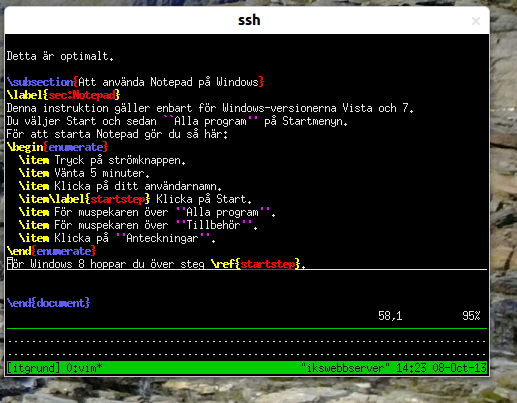
\includegraphics[height=7cm]{vim.png}
  \caption{En skärmdump av en trevlig session i denna utomordentliga 
  textredigerare.}
  \label{fig:vim}
\end{figure}

\subsection{Att använda Notepad på Windows}
\label{sec:Notepad}
Denna instruktion gäller enbart för Windows-versionerna Vista och 7.
Du väljer Start och sedan ``Alla program'' på Startmenyn.
För att starta Notepad gör du så här:
\begin{enumerate}
  \item Tryck på strömknappen.
  \item Vänta 5 minuter.
  \item Klicka på ditt användarnamn.
  \item\label{startstep} Klicka på Start.
  \item För muspekaren över ''Alla program''.
  \item För muspekaren över ''Tillbehör''.
  \item Klicka på ''Anteckningar''.
\end{enumerate}
För Windows 8 hoppar du över steg \ref{startstep}.

\subsection{Övriga textredigerare}
\label{sec:misc}
Det finns många olika textredigerare.
Du finner några exempel i tabell \ref{tab:editors}.

\begin{table}
  \centering
  \begin{tabular}{l|l}
    \textbf{Kommando}   & \textbf{Operativsystem} \\
    \hline
    vim                 & Alla UNIX-lika system, Windows \\
    sublime             & Alla UNIX-lika system, Windows \\
    Notepad             & Enbart Windows \\
    gedit               & UNIX-lika system under Gnome \\
    notepad++           & Windows \\
    nano                & Alla UNIX-lika system \\
    emacs               & Alla UNIX-lika och Windows, men använd hellre vim \\
  \end{tabular}
  \caption{En tabell över några vanliga textredigerare och vilka operativsystem 
  dessa finns tillgängliga för.}
  \label{tab:editors}
\end{table}


\section{Datorn}
\label{sec:computer}
En dator är avancerad, se exempelvis Brookshears bok om datavetenskap 
\cite{Brookshear2012csa}.
I den beskriver Brookshear att ''[a]n important task of an operating system is 
the allocation of the machine's resources to the processes in the system'' 
\cite[sidan 139]{Brookshear2012csa}.


\bibliography{literature}
\end{document}

% här finns normalt ingenting
